\chapter*{Acknowledgement}
% \chaptermark{Acknowledgement}

Je tiens à remercier mes encadrants Nicolas Courty, Rémi Flamary et Karim Lounici.
C'était en Décembre 2021 que je vous ai contacté pour une thèse.
Vous m'avez donné la chance de découvrir le transport optimal pendant la période très difficile de la pandémie.
Rémi, le fait que t'es non seulement un superbe prof, mais aussi un superbe psychologue. Apart de la discussion
sur la science, je ne peux pas compter combien de fois je te laisse souffler mon "impostor syndrome".
Mais t'es toujours là pour les conseils, avec la patience et la sympathie.
Merci Nicolas de m'avoir accueilli plusieurs fois à Vannes. Il n'y a pas que les séminaires
Dès la première visite, j'avais toujours des regrets de n'avoir pas pu déménager à Vannes
(sorry Rémi ...). J'aurai un cadeau spécial pour toi, let's see what it is :).
Une visite est littéralement une nouvelle idée.
Encore une fois, un grand merci et une grande gratitude à vous.

I would like to thank Facundo Mémoli and François-Xavier Vialard for their report and
time reading the manuscript. Their feedbacks have helped improve
I would also like to thank Laetitial Chapel, Alain Durmus and Gabriel Peyré
for accepting to be members of the jury. It is a honor to present i

Je souhaite remercier Ievgen. Grâce à toi, j'ai une très belle collaboration
avec l'équipe de Pinar et Ritambhara. J'ai l'ocassion de découvrir les superbes
applications de COOT en single-cell multi-omics. Fun fact: t'es le seul coauteur qui
apparait dans toutes mes publications pendant ma thèse :).

I would like to thank. my parents.. \\
J'adresse également toute ma reconnaissance à .... \\

Alexis, c'est toujours un plaisir de travailler avec toi.
Je n'oublierai jamais les journées qu'on a débuggé FUGW dans ton bureau à Collège de France.
Puis, après la discussion sur la science, on a parlé de la vie et
gouté les cuisines chinoise, grèce, vietnamienne dans ton quartier Latin.

Merci Clément, pour .
Merci les Télécommiens Paul, Hicham, Arturo, Binh
Merci mes amis vietnamiens dans le groupe Math en France, pour les supports
techniques et aussi la motivation. Merci anh Tan et

A ma chérie, ma femme: on avait des moments difficiles mais au final,
on a réussi à les surmontés.
Je suis content et que t'es toujours avec moi. Mon amour pour toi,
et pour nos chats Ti et Bun.

\begin{figure}[t]
    \centering
    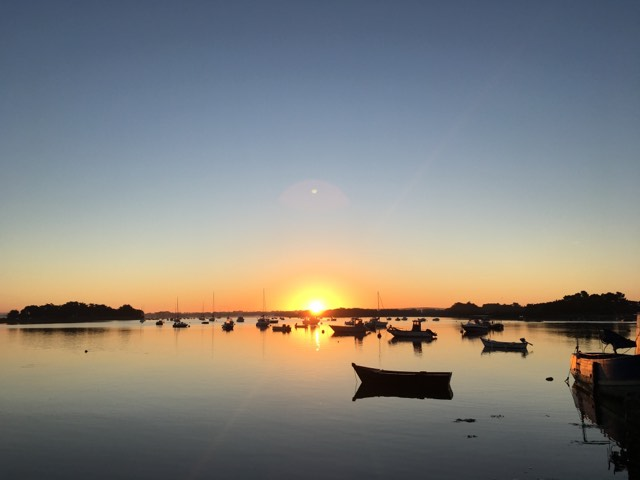
\includegraphics[width=0.7\linewidth]{./Chapitre0/sunrise_vannes.jpg}
    \caption*{Sunrise in Vannes, 24 September 2021}
\end{figure}
